Considera la funció
\[
f(x)=\begin{cases}
  e^{x+1}+1 & \si{x<-1},\\[4pt]
  x^2+1 & \si{-1\le x\le 1},\\[4pt]
  \dfrac{4}{x+1} & \si{x>1}.
\end{cases}
\]

\begin{apartats}

\apartat[1,25]{1}
Estudia'n la continuïtat i troba'n les asímptotes.

\begin{solucio}
Cada branca és contínua al seu tros: el denominador de la tercera s'anul·la en $x=-1$, que no és al
seu tros.\\
En $x=-1$: $\lim_{x\to-1^-}f(x)=e^0+1=2$ i $f(-1)=2$. En $x=1$: $f(1)=2$ i
$\lim_{x\to1^+}f(x)=\dfrac42=2$. La funció és \textbf{contínua a tot $\mathbb{R}$}.\\
\textbf{Asímptotes verticals}: cap. \textbf{Horitzontals}: per l'esquerra,
$\lim_{x\to-\infty}f(x)=0+1=1$, i per la dreta, $\lim_{x\to+\infty}f(x)=0$. Té \textbf{dues}
asímptotes horitzontals diferents: $y=1$ per l'esquerra i $y=0$ per la dreta.
\end{solucio}

\begin{nomesllarg}
\apartat{0,75}
Estudia'n la monotonia i troba'n els extrems.

\begin{solucio}
Per a $x<-1$: $f'(x)=e^{x+1}>0$, creix. Per a $-1<x<1$: $f'(x)=2x$, decreix a $(-1,0)$ i creix a
$(0,1)$. Per a $x>1$: $f'(x)=\dfrac{-4}{(x+1)^2}<0$, decreix.\\
\textbf{Màxims relatius} $(-1,2)$ i $(1,2)$, i \textbf{mínim relatiu} $(0,1)$. En $x=\pm1$ la funció
no és derivable (les derivades laterals hi valen $1$ i $-2$, i $2$ i $-1$), però sí que hi té un
màxim: la gràfica hi fa un angle.
\end{solucio}
\end{nomesllarg}

\begin{tria}{trossos-tasca}
\itemtria{original}{0,75}{1,25}
Representa la funció.

\begin{solucio}
Ve de prop de $y=1$, puja fins al màxim $(-1,2)$, baixa fins al mínim $(0,1)$, torna a pujar fins al
màxim $(1,2)$ i, des d'allà, baixa cap a l'eix $OX$ sense arribar-hi mai. No talla l'eix $OX$, i
talla l'eix $OY$ en $(0,1)$.
\begin{center}
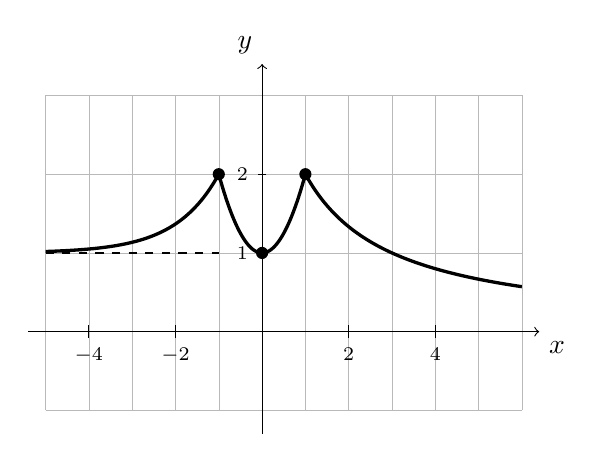
\begin{tikzpicture}[x=0.55cm,y=1cm]
  \draw[gray!55,very thin,step=1] (-5,-1) grid (6,3);
  \draw[->] (-5.4,0) -- (6.4,0) node[below right] {$x$};
  \draw[->] (0,-1.3) -- (0,3.4) node[above left] {$y$};
  \foreach \i in {-4,-2,2,4} \draw (\i,0.08) -- (\i,-0.08) node[below,font=\scriptsize] {$\i$};
  \foreach \j in {1,2} \draw (0.1,\j) -- (-0.1,\j) node[left,font=\scriptsize] {$\j$};
  \draw[dashed,thick] (-5,1) -- (-1,1);
  \begin{scope}
    \clip (-5,-1) rectangle (6,3);
    \draw[\colorgrafica,very thick,domain=-5:-1,samples=80,smooth] plot (\x,{exp(\x+1)+1});
    \draw[\colorgrafica,very thick,domain=-1:1,samples=60,smooth] plot (\x,{\x*\x+1});
    \draw[\colorgrafica,very thick,domain=1:6,samples=80,smooth] plot (\x,{4/(\x+1)});
  \end{scope}
  \fill (-1,2) circle (2.2pt); \fill (0,1) circle (2.2pt); \fill (1,2) circle (2.2pt);
\end{tikzpicture}
\end{center}
\end{solucio}

\itemtria{extrems-absoluts}{0,75}{1,25}
Té $f$ un màxim absolut? I un mínim absolut? Justifica-ho a partir de la monotonia i de les
asímptotes.

\begin{solucio}
$f$ creix a $(-\infty,-1)$, decreix a $(-1,0)$, creix a $(0,1)$ i decreix a $(1,+\infty)$, amb
$f(-1)=f(1)=2$ i $f(0)=1$.\\
A l'esquerra, els valors són de $(1,2)$, perquè s'acosten a l'asímptota $y=1$; al mig, de $[1,2]$; i a
la dreta, de $(0,2)$, perquè s'acosten a $y=0$. Per tant, $f(x)\le2$ sempre: el \textbf{màxim absolut}
és $2$, i s'assoleix dues vegades, en $x=-1$ i en $x=1$.\\
\textbf{Mínim absolut}: no n'hi ha. $f(x)>0$ sempre, però s'acosta a $0$ tant com es vulgui quan
$x\to+\infty$, sense arribar-hi mai. El mínim relatiu, $(0,1)$, no és l'absolut: per a $x>3$, la
tercera branca val menys d'$1$. El recorregut és $(0,2]$.
\end{solucio}
\end{tria}

\end{apartats}
